\chapter{System Build and Estimation}
\label{ch:estimation}

The formulas of Chapter~\ref{ch:methods} do not, by themselves, say whether the two technologies move the five targets. This chapter builds the smallest system that can be run, and then estimates it. Section~\ref{sec:build} describes the cell, the data, the programs, and the way RCH-GAT and SSDT-CC sit inside them. Section~\ref{sec:estimate} reports what those programs produced on four stresses of the order book, on two ablations, and on a sweep of the chance-constraint tolerance. The estimates are means and standard deviations over paired random order books. They are not measurements from a physical sewing line, and the text does not treat them as if they were.

\section{System build}
\label{sec:build}

\subsection{What was built}

The system is a discrete-event shop cell and a dispatcher that share one state. The cell holds orders, machines, operators, dies, and thread lots. The dispatcher is called whenever the cell has a free feasible bundle. It returns one bundle, optionally prefixed by preventive maintenance. The cell advances that bundle, writes the new health, releases the resources at the end, and calls the dispatcher again. There is no nightly plan file. Figure~\ref{fig:architecture} is the whole architecture.

\begin{figure}[ht]
\centering
\begin{tikzpicture}[
  box/.style={draw, rounded corners, align=center, font=\small, minimum width=2.7cm, minimum height=0.9cm},
  arr/.style={-{Stealth}, thick}
]
\node[box] (ord) {Order book\\releases, routes};
\node[box, right=1.0cm of ord] (cell) {Shop cell\\machines, people, tokens};
\node[box, right=1.0cm of cell] (twin) {Twin\\health and \(\phi\)};
\node[box, below=1.05cm of twin] (pol) {RCH-GAT\\masked score};
\node[box, below=1.05cm of cell] (log) {KPI log\\five targets};
\draw[arr] (ord) -- (cell);
\draw[arr] (cell) -- (twin);
\draw[arr] (twin) -- (pol);
\draw[arr] (pol) -- (cell);
\draw[arr] (cell) -- (log);
\end{tikzpicture}
\caption{Executable architecture. The policy reads the twin and writes one bundle back into the cell. The KPI log is the only path from a run to the tables in Section~\ref{sec:estimate}.}
\label{fig:architecture}
\end{figure}

Four programs implement the figure. The shop generator builds an order book from a seed and a scenario name. The cell executes Algorithm~\ref{alg:dispatch}. The scorer evaluates Equation~\eqref{eq:psi} and Algorithm~\ref{alg:ssdt}. The identification program runs Algorithm~\ref{alg:cem} and stores the coefficient vector. A comparison driver repeats the cell for every method, every scenario, and every seed, and writes the means. The driver is deterministic given the seed. Re-running it reproduces the tables.

The cell is the plant. It is also the sensor, in the sense of Section~\ref{sec:ssdt}: health is updated by the wear recursion \eqref{eq:plant-wear} rather than by a Kalman correction of a noisy current trace. That choice is deliberate. It removes sensor luck from the comparison. It does not remove the status effect, because wear, the duration factor, the hazard, and the maintenance map are all active.

\subsection{The cell}

Nine machines form seven groups. Table~\ref{tab:machines} lists the quantities that enter Equations~\eqref{eq:ptime} and \eqref{eq:f3}. Health at the start of the day is part of the scenario, not a warm-up artefact. Cutter-A is fast, powerful, and already at \(0.58\). Lockstitch-2 is at \(0.52\). The embroidery head is at \(0.46\). A scheduler that ignores status is ignoring the largest machines in the cell, not a rounding error on a healthy fleet.

\begin{table}[ht]
\centering
\caption{Machines in the estimation cell. Wear is the drift \(\eta_k\) in health per processing minute. Health \(h_0\) is the nominal-scenario initial state.}
\label{tab:machines}
\small
\begin{tabular}{llrrrr}
\toprule
Machine & Group & Power (kW) & Speed & Wear & \(h_0\) \\
\midrule
Cutter-A & cut & 6.8 & 1.28 & 0.00115 & 0.58 \\
Cutter-B & cut & 2.4 & 0.74 & 0.00055 & 0.22 \\
Embroidery-1 & print & 3.4 & 1.00 & 0.00050 & 0.46 \\
Lockstitch-1 & sew & 0.75 & 1.05 & 0.00038 & 0.24 \\
Lockstitch-2 & sew & 0.75 & 0.98 & 0.00040 & 0.52 \\
Bartack-1 & sew, heavy & 1.15 & 1.00 & 0.00048 & 0.34 \\
Hardware-1 & hardware & 1.45 & 1.00 & 0.00028 & 0.20 \\
QC-1 & inspect & 0.35 & 1.00 & 0.00008 & 0.08 \\
Pack-1 & pack & 0.55 & 1.00 & 0.00008 & 0.12 \\
\bottomrule
\end{tabular}
\end{table}

Eight operators staff the nine machines, which is the dual-resource constraint. Table~\ref{tab:operators} is the skill matrix. A blank entry is a hard zero and is masked. Cut-2 can pack slowly and is the only second cutter. Print-1 is the only embroidery operator and can stand in at inspection. Sew-3 cannot run the bartack. The hardware operator and the inspection operator both reach the packing table, so packing is rarely the resource that deadlocks, and hardware sometimes is.

\begin{table}[ht]
\centering
\caption{Operator skills. The number multiplies machine speed in Equation~\eqref{eq:ptime}. A dash is an infeasible pairing.}
\label{tab:operators}
\small
\begin{tabular}{lrrrrrrr}
\toprule
Operator & Cut & Print & Sew & Heavy & Hardware & Inspect & Pack \\
\midrule
Cut-1 & 1.00 & -- & -- & -- & -- & -- & -- \\
Cut-2 & 0.82 & -- & -- & -- & -- & -- & 0.55 \\
Print-1 & -- & 1.00 & -- & -- & -- & 0.45 & -- \\
Sew-1 & -- & -- & 1.06 & 0.78 & -- & -- & -- \\
Sew-2 & -- & -- & 0.96 & 1.08 & -- & -- & -- \\
Sew-3 & -- & -- & 1.00 & -- & -- & -- & -- \\
Hard-1 & -- & -- & -- & -- & 1.00 & -- & 0.70 \\
QC-1 & -- & -- & -- & -- & 0.62 & 1.00 & 0.95 \\
\bottomrule
\end{tabular}
\end{table}

Tokens are few on purpose. Two dies cover two cutters. Thread lots allow two concurrent users of navy, black, red, and grey, and one user of khaki. In the shortage scenario the navy, red, and khaki pools drop to one. Colour setup is eleven minutes on cutting, embroidery, and sewing when the previous colour differs, and four minutes when the machine has no remembered colour. The repair expectation, when a failure probability is priced, is forty-eight minutes at half nameplate power. Preventive maintenance, when the chance constraint fires, is sixteen minutes and applies Equation~\eqref{eq:pm-map}.

Routes are those of Section~\ref{sec:problem-set}. A backpack has eight operations, a trolley bag seven, and a sports sack six. Base minutes at quantity 80 and size M are stored with the route. A random order draws a style, a colour, a size in \(\{S,M,L\}\), a quantity in \(\{40,60,80,100,120\}\), a release time in \(\{0,40,90,150\}\) minutes, and a due date equal to the release time plus a multiple of the route's base work. The multiple is drawn uniformly from \(3.6\) to \(6.4\), which is wide enough that a good schedule can finish a substantial share of orders on time and a poor schedule cannot. Sixteen orders form a book, except in the rush scenario, which adds four more at time \(220\).

\subsection{Methods that share the cell}

Every method uses the same cell, the same mask, and the same health plant. They differ in the ranking of feasible bundles and in whether Algorithm~\ref{alg:ssdt} is allowed to maintain.

First-in-first-out ranks by release time, then by order identity, then by operation index. Shortest processing time ranks by processing time plus setup, using the health-scaled time of Equation~\eqref{eq:ptime}, because hiding health inside the baseline's clock and not inside its ranking would invent a gain. The baselines are allowed to see the true processing time. They are not given the failure features, the token-contention features, or the maintenance action. Earliest due date ranks by \(d_j\). Apparent tardiness cost uses Equation~\eqref{eq:atc} with look-ahead \(k = 2\) and a forty-minute average processing time.

RCH is Equation~\eqref{eq:psi} with the identified coefficients and with the maintenance test switched off. RCH-SSDT is the same score with the test switched on at \(\varepsilon = 0.10\). The no-resource ablation zeroes the contention costs \(\rho_9,\rho_{10},\rho_{11}\) and the shop-node key, and still allows maintenance. The no-status ablation zeroes health and failure in the score and switches maintenance off. The plant's wear and the plant's expected repair delay remain active for every method, including the ablations. Otherwise a method that ``ignores status'' would be running a different factory.

An evolutionary reference is reported separately and is not given maintenance. On four nominal books a small NSGA-II \cite{deb2002}, with a population of eighteen and twelve generations, searches a priority key per operation and a machine bias. The decoder is the same cell. The front it returns is a static search on one book, not an online policy. It is there to show what a short population search can move when it is allowed to look at the whole book at once, and what it does not move when it cannot renew a machine.

\subsection{Identification}

Coefficients were identified on four books, seeds \(11\), \(23\), \(37\), and \(41\), which are not in the estimation seeds. The preference during identification was the balanced vector \(\omega = (0.34, 0.33, 0.18, 0.15)\), ordered as makespan, tardiness, energy, and imbalance, with the failure ratio added at weight \(0.12\) as in Equation~\eqref{eq:scalar}. The cross-entropy search used a population of \(36\), an elite of \(8\), and \(28\) generations. Figure~\ref{fig:train} shows the best and the mean fitness. Fitness is \(J_\omega\) relative to first-in-first-out, so a value of one is a tie with that rule and a value below one is an improvement on the scalar.

\begin{figure}[ht]
\centering
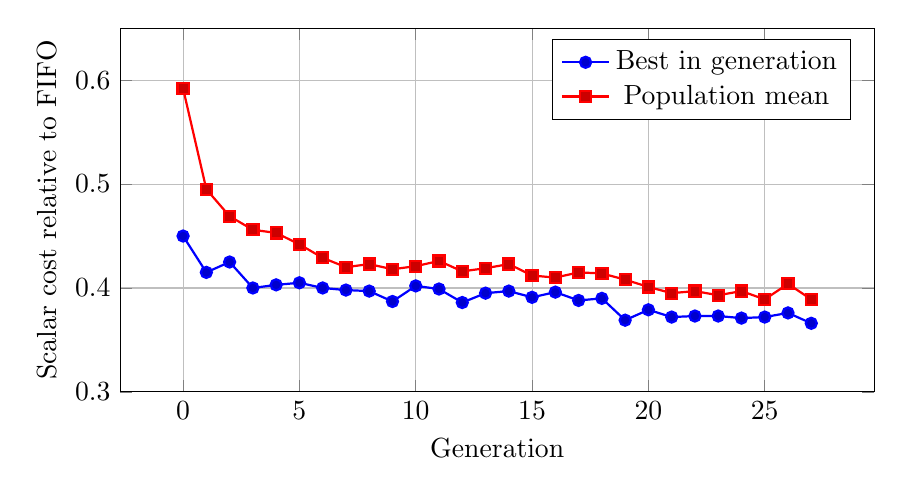
\begin{tikzpicture}
\begin{axis}[
  width=0.92\textwidth,
  height=6.2cm,
  xlabel={Generation},
  ylabel={Scalar cost relative to FIFO},
  ymin=0.30, ymax=0.65,
  legend pos=north east,
  grid=both,
  every axis plot/.append style={thick}
]
\addplot coordinates {
(0,0.450) (1,0.415) (2,0.425) (3,0.400) (4,0.403) (5,0.405)
(6,0.400) (7,0.398) (8,0.397) (9,0.387) (10,0.402) (11,0.399)
(12,0.386) (13,0.395) (14,0.397) (15,0.391) (16,0.396) (17,0.388)
(18,0.390) (19,0.369) (20,0.379) (21,0.372) (22,0.373) (23,0.373)
(24,0.371) (25,0.372) (26,0.376) (27,0.366)
};
\addlegendentry{Best in generation}
\addplot coordinates {
(0,0.592) (1,0.495) (2,0.469) (3,0.456) (4,0.453) (5,0.442)
(6,0.429) (7,0.420) (8,0.423) (9,0.418) (10,0.421) (11,0.426)
(12,0.416) (13,0.419) (14,0.423) (15,0.412) (16,0.410) (17,0.415)
(18,0.414) (19,0.408) (20,0.401) (21,0.395) (22,0.397) (23,0.393)
(24,0.397) (25,0.389) (26,0.404) (27,0.389)
};
\addlegendentry{Population mean}
\end{axis}
\end{tikzpicture}
\caption{Identification of the twenty score coefficients. The vertical axis is the preference-weighted cost divided, term by term, by first-in-first-out on the same training books. The search was stopped at generation 27. The coefficient vector used in the tables is the best vector observed, at \(0.366\).}
\label{fig:train}
\end{figure}

The curve falls quickly and then flattens. Most of the scalar gain is present by generation ten. Later generations trim the best value from about \(0.39\) to \(0.366\) and do not change the identity of the method. This is the behaviour one expects when the score is a low-dimensional monotone function of sensible costs and the mask already carries the combinatorial structure. It is not evidence that a deep multi-layer network would be unnecessary on a plant with hundreds of machines. It is evidence that, on this cell, the attention score of Section~\ref{sec:rch} can be identified without hiding the result inside an opaque training run.

\subsection{Scenarios and the statistics that are reported}

Four scenarios stress the problem set.

The nominal scenario is the cell as tabulated, with sixteen orders and the standard token capacities. It is the fair day.

The rush scenario releases four extra orders at minute \(220\), with due dates at \(2.15\) times their base work after that release. They are tighter than the ordinary multiple of \(3.6\) to \(6.4\). Every online method, including the classical rules, can see them only after minute \(220\). The scenario asks whether rebuilding the feasible set, which all online methods do, is enough, or whether the score and the twin still matter once the book has grown.

The wear scenario multiplies every wear rate by \(1.85\) and adds \(0.10\) to every initial health. Cutter-A then starts at \(0.68\), already deep into the hazard. This is the scenario the twin is for.

The shortage scenario leaves wear nominal and cuts the navy, red, and khaki pools to one concurrent user. This is the scenario the shop node is for.

Each scenario is run on twenty books, seeds \(1000\) through \(1019\), paired across methods. Tables report the mean and, in the text, the standard deviation. Total tardiness has a large standard deviation because one late trolley bag dominates the sum. A difference of a few tens of minutes in mean tardiness, against a standard deviation of a few hundreds, is reported as a point estimate and is not promoted to a ranking. Differences that exceed the spread, in particular makespan, energy, and expected failures for the full system against the classical rules, are treated as the estimation's actual findings.

The failure column is an expectation, summed from Equation~\eqref{eq:phi}. Two methods can be compared on it without a second random draw. Expected repair minutes are inserted into the timeline so that a method which accepts a high \(\phi\) also accepts the blocking time that follows.

\section{Estimation}
\label{sec:estimate}

\subsection{Nominal book}

Table~\ref{tab:nominal} is the main estimate. Times are minutes. Energy is kilowatt-hours. Failures are the expected count \(f_5\). On-time rate is the fraction of orders with no tardiness. The twenty-book standard deviation of makespan is about \(166\) minutes for first-in-first-out and about \(83\) minutes for the full system. The standard deviation of tardiness is several hundred minutes for every method.

\begin{table}[ht]
\centering
\caption{Nominal order books, twenty paired seeds. Lower is better except for the on-time rate.}
\label{tab:nominal}
\small
\begin{tabular}{lrrrrrrr}
\toprule
Method & Makespan & Tardiness & On time & Energy & Imbalance & Failures & PM \\
\midrule
FIFO & 1520.7 & 2761.4 & 0.519 & 303.2 & 377.7 & 18.02 & 0 \\
SPT & 1547.6 & 512.8 & 0.816 & 268.3 & 366.0 & 15.56 & 0 \\
EDD & 1545.4 & 212.1 & 0.891 & 299.3 & 377.4 & 16.95 & 0 \\
ATC & 1631.8 & 274.7 & 0.863 & 299.1 & 393.8 & 17.44 & 0 \\
RCH & 1234.4 & 260.9 & 0.853 & 211.0 & 260.4 & 10.13 & 0 \\
RCH-SSDT & 1051.6 & 165.1 & 0.903 & 167.5 & 222.1 & 0.91 & 5.35 \\
No resource & 1050.6 & 135.4 & 0.903 & 168.2 & 218.6 & 0.89 & 5.70 \\
No status & 1260.4 & 268.5 & 0.875 & 207.7 & 263.8 & 10.22 & 0 \\
\bottomrule
\end{tabular}
\end{table}

Read the classical block first. First-in-first-out finishes about half the orders on time and accumulates \(2761\) minutes of tardiness. Shortest processing time and earliest due date cut that tardiness sharply, to \(513\) and \(212\) minutes, and they do not cut the makespan. All four rules finish the day in roughly \(1520\) to \(1632\) minutes and burn roughly \(268\) to \(303\,\mathrm{kWh}\). Expected failures sit between \(15.6\) and \(18.0\). Apparent tardiness cost does not beat earliest due date on this book. The look-ahead in Equation~\eqref{eq:atc} is a good idea on a pure tardiness problem and is not, here, a substitute for health and tokens.

RCH, which is the graph score without maintenance, is the estimate of the first technology alone. Makespan falls from \(1520.7\) to \(1234.4\) minutes, a reduction of \(286\) minutes against first-in-first-out and of about \(310\) minutes against earliest due date. Energy falls from the best classical value, the \(268.3\,\mathrm{kWh}\) of shortest processing time, to \(211.0\,\mathrm{kWh}\). Imbalance falls from about \(370\) to \(260\). Expected failures fall from about \(16\) to \(10.1\). Tardiness, at \(260.9\) minutes, is better than shortest processing time and worse, as a point estimate, than earliest due date's \(212.1\). The on-time rates are \(0.85\) and \(0.89\). Given tardiness standard deviations of \(250\) and \(356\) minutes, that ordering is not a stable ranking. The honest nominal statement about RCH is that it shortens the day, saves energy, balances the machines, and avoids some failures, while staying in the same tardiness band as the due-date rules.

RCH-SSDT is the estimate of the two technologies together. Makespan falls further, to \(1051.6\) minutes. Energy falls to \(167.5\,\mathrm{kWh}\). Expected failures fall to \(0.91\), with \(5.35\) preventive maintenances on an average book. Expected breakdown delay, which is \(865\) minutes under first-in-first-out and \(486\) minutes under RCH, is \(44\) minutes under the full system. Tardiness' point estimate, \(165\) minutes, is below earliest due date, and the on-time rate is \(0.90\). The tardiness standard deviation is still \(205\) minutes, so the due-date claim is the weak one. The makespan, energy, failure, and balance claims are not weak: the full system's makespan spread (\(\pm 83\)) and the classical makespan spread (\(\pm 150\) or more) do not cover a gap of about \(470\) minutes, and the failure gap is from the teens to under one.

The ablations split the gain. Removing status features and maintenance returns the result to the RCH band: makespan \(1260\), energy \(208\), failures \(10.2\). The twin, not the attention biases, is what drives failures from ten to under one. Removing resource features and keeping maintenance does not hurt the nominal book. The point estimates of makespan and energy stay inside a few minutes of the full system, and the tardiness point estimate is even lower. Token pools of two, on a sixteen-order nominal book, are not tight enough for the shop node to earn its keep. That is a finding about this scenario, not a reason to delete the node. The shortage and rush scenarios are where the node was supposed to matter, and they are reported next.

Figure~\ref{fig:bars} repeats the four headline means so the gap is visible without the full table.

\begin{figure}[ht]
\centering
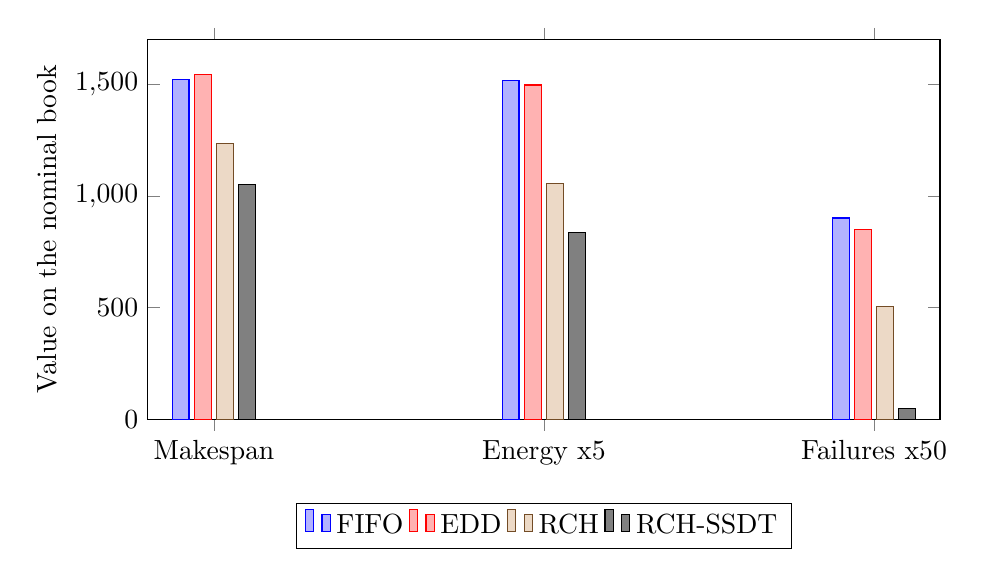
\begin{tikzpicture}
\begin{axis}[
  width=0.96\textwidth,
  height=6.4cm,
  ybar,
  bar width=6pt,
  ylabel={Value on the nominal book},
  symbolic x coords={Makespan, Energy x5, Failures x50},
  xtick=data,
  ymin=0,
  legend style={at={(0.5,-0.22)}, anchor=north, legend columns=4},
  nodes near coords style={font=\tiny},
  every node near coord/.append style={font=\tiny}
]
\addplot coordinates {(Makespan,1521) (Energy x5,1516) (Failures x50,901)};
\addplot coordinates {(Makespan,1545) (Energy x5,1497) (Failures x50,848)};
\addplot coordinates {(Makespan,1234) (Energy x5,1055) (Failures x50,506)};
\addplot coordinates {(Makespan,1052) (Energy x5,838) (Failures x50,46)};
\legend{FIFO, EDD, RCH, RCH-SSDT}
\end{axis}
\end{tikzpicture}
\caption{Nominal means rescaled onto one axis. Energy is multiplied by five and expected failures by fifty, so that a kilowatt-hour and a failure can sit beside a minute of makespan. The scaling is only for the drawing. Table~\ref{tab:nominal} has the unscaled numbers.}
\label{fig:bars}
\end{figure}

\subsection{Rush release}

Table~\ref{tab:rush} adds four orders at minute \(220\). The day is longer for every method, and tardiness grows because the new due dates are tight and because the embroidery head and the hardware bench were not idle.

\begin{table}[ht]
\centering
\caption{Rush release at minute 220, twenty paired seeds. The book contains twenty orders after the release.}
\label{tab:rush}
\small
\begin{tabular}{lrrrrrr}
\toprule
Method & Makespan & Tardiness & On time & Energy & Failures & PM \\
\midrule
FIFO & 2013.0 & 7701.6 & 0.415 & 416.9 & 30.24 & 0 \\
SPT & 1928.5 & 3090.4 & 0.515 & 356.0 & 24.30 & 0 \\
EDD & 2001.5 & 2716.0 & 0.425 & 408.2 & 27.39 & 0 \\
ATC & 2008.1 & 2871.0 & 0.410 & 403.1 & 27.11 & 0 \\
RCH & 1676.1 & 1577.6 & 0.495 & 302.4 & 17.93 & 0 \\
RCH-SSDT & 1264.6 & 735.5 & 0.685 & 214.6 & 1.02 & 7.85 \\
No resource & 1274.9 & 805.8 & 0.708 & 213.0 & 1.02 & 7.70 \\
No status & 1597.5 & 1473.6 & 0.557 & 298.0 & 17.15 & 0 \\
\bottomrule
\end{tabular}
\end{table}

Earliest due date, which won the nominal tardiness point estimate, now records \(2716\) minutes of tardiness and an on-time rate of \(0.43\). The rule does see the rush orders. Seeing them is not the same as placing them onto a machine that will still be healthy when they arrive. Shortest processing time is similar, with a slightly shorter day and slightly less energy, and with tardiness still near \(3100\) minutes. Standard deviations of rush tardiness are about \(900\) to \(1300\) minutes for the classical rules and \(522\) minutes for the full system. The gap from \(2716\) to \(736\) is large beside those spreads. The on-time rate moves from \(0.43\) to \(0.69\).

The full system finishes in \(1265\) minutes instead of about \(2000\), at \(215\,\mathrm{kWh}\) instead of about \(400\), with one expected failure instead of about twenty-seven, using \(7.9\) maintenances. RCH without maintenance already reaches \(1676\) minutes, \(302\,\mathrm{kWh}\), and \(17.9\) expected failures, so the graph score is doing part of the work before the twin renews anything. The no-status ablation sits next to that RCH result. The no-resource ablation sits next to the full system and is a little worse on makespan and on the tardiness point estimate (\(1275\) and \(806\) against \(1265\) and \(736\)). The resource features point the right way under a rush, and the difference is much smaller than the difference made by maintenance. A rush overloads machines and health before it overloads token pools.

\subsection{Accelerated wear}

Table~\ref{tab:wear} is the twin's scenario. Initial health is higher and every processing minute writes more wear.

\begin{table}[ht]
\centering
\caption{Accelerated wear, twenty paired seeds. Initial health is shifted up by \(0.10\) and every wear coefficient is multiplied by \(1.85\).}
\label{tab:wear}
\small
\begin{tabular}{lrrrrrr}
\toprule
Method & Makespan & Tardiness & On time & Energy & Failures & PM \\
\midrule
FIFO & 2097.7 & 5898.7 & 0.397 & 388.2 & 42.26 & 0 \\
SPT & 2034.0 & 2093.5 & 0.641 & 351.7 & 36.24 & 0 \\
EDD & 2059.3 & 1849.0 & 0.584 & 384.3 & 38.75 & 0 \\
ATC & 2120.8 & 2252.4 & 0.547 & 382.0 & 38.91 & 0 \\
RCH & 1782.0 & 895.1 & 0.697 & 310.0 & 30.58 & 0 \\
RCH-SSDT & 1121.7 & 287.2 & 0.850 & 176.1 & 0.81 & 11.95 \\
No resource & 1109.8 & 279.5 & 0.831 & 174.6 & 0.83 & 11.85 \\
No status & 1676.9 & 1054.7 & 0.706 & 283.6 & 28.88 & 0 \\
\bottomrule
\end{tabular}
\end{table}

Without maintenance the day runs away. Classical makespans sit near \(2100\) minutes, with \(36\) to \(42\) expected failures and about \(1700\) to \(2000\) minutes of expected repair delay charged into the timeline. RCH, which can see health and still cannot renew it, improves the book to \(1782\) minutes and \(30.6\) expected failures. Seeing the worn cutter and preferring the healthy one is worth several hundred minutes. It is not worth what renewal is worth.

With the chance constraint on, the same books finish in \(1122\) minutes, at \(176\,\mathrm{kWh}\), with \(0.81\) expected failures and \(12.0\) maintenances. The no-status ablation, at \(1677\) minutes and \(28.9\) expected failures, confirms that the score's health features without the maintenance action do not reproduce this result. The no-resource ablation is statistically the same as the full system on this scenario. Wear does not act through the khaki lot.

Twelve maintenances of sixteen minutes are \(192\) minutes of tool-change time. The expected repair delay avoided, relative to earliest due date, is about \(1860 - 39 = 1821\) minutes. The arithmetic of Table~\ref{tab:worked} was that one maintenance does not pay for itself inside one cycle. The arithmetic of Table~\ref{tab:wear} is that the same action, applied when the test fires, pays for itself across the day by a wide margin. Both statements are true. They refer to different horizons, which is why the twin is a day-level technology even though its test is a cycle-level test.

Tardiness follows the makespan. The full system's point estimate is \(287\) minutes and its on-time rate is \(0.85\), against \(1849\) minutes and \(0.58\) for earliest due date. The tardiness standard deviation is \(364\) minutes for the full system and \(1009\) for earliest due date. The gap remains large beside those spreads. This is the scenario in which the due-date claim is actually supported, because the failures that the due-date rule accepts are what make the orders late.

\subsection{Thread-lot shortage}

Table~\ref{tab:shortage} restores nominal wear and tightens three colour pools to a single concurrent user.

\begin{table}[ht]
\centering
\caption{Thread-lot shortage, twenty paired seeds. Navy, red, and khaki allow only one concurrent user.}
\label{tab:shortage}
\small
\begin{tabular}{lrrrrrr}
\toprule
Method & Makespan & Tardiness & On time & Energy & Failures & PM \\
\midrule
FIFO & 1456.0 & 2329.7 & 0.544 & 295.5 & 15.85 & 0 \\
SPT & 1462.0 & 350.7 & 0.850 & 260.0 & 13.47 & 0 \\
EDD & 1515.9 & 162.6 & 0.925 & 290.8 & 14.74 & 0 \\
ATC & 1564.0 & 219.2 & 0.916 & 289.2 & 15.01 & 0 \\
RCH & 1225.4 & 171.4 & 0.887 & 208.2 & 9.29 & 0 \\
RCH-SSDT & 1038.7 & 106.3 & 0.925 & 163.5 & 0.76 & 5.15 \\
No resource & 1074.6 & 113.0 & 0.938 & 165.4 & 0.79 & 5.30 \\
No status & 1204.6 & 220.6 & 0.891 & 203.2 & 9.01 & 0 \\
\bottomrule
\end{tabular}
\end{table}

The pattern of the nominal book returns, with one extra detail. The full system is again shorter, cooler, and almost free of expected failures: \(1039\) minutes, \(164\,\mathrm{kWh}\), \(0.76\) failures, on-time rate \(0.93\). Earliest due date matches the on-time rate and loses more than \(470\) minutes of makespan and about \(127\,\mathrm{kWh}\). RCH without maintenance sits in between, as before.

The resource ablation is the detail. Without contention features the makespan point estimate rises from \(1038.7\) to \(1074.6\) and tardiness from \(106.3\) to \(113.0\). The standard deviations are about \(90\) minutes of makespan and about \(150\) minutes of tardiness, so a \(36\)-minute makespan gap is a shift of the mean, not a separation that a single book would reliably show. It is, however, in the direction the shop node was built for, and it appears under shortage and, with a similar size, under rush, while it does not appear under nominal tokens or under pure wear. The estimation therefore supports a limited claim. Resource features are a small, correctly signed correction when lots are tight, and they are not the source of the large gains in makespan, energy, and failures. Those gains survive the ablation. A factory that already has ample dies and thread, and that is trying to justify the shop node alone, will not see them in a one-day book of this size. A factory whose khaki lot is a single spool will see a modest tightening of the day, on top of the much larger tightening that comes from not running the cutter into a repair.

\subsection{The tolerance as a knob}

The wear scenario was repeated on eight further books for five values of \(\varepsilon\). These seeds are not the twenty books of Table~\ref{tab:wear}, so the row \(\varepsilon = 0.10\) does not reproduce that table's mean exactly. The sweep is a curve, not a second copy of the main experiment. Table~\ref{tab:eps} and Figure~\ref{fig:eps} report it.

\begin{table}[ht]
\centering
\caption{Chance-constraint tolerance on eight accelerated-wear books. The policy is RCH-SSDT. Maintenance count is the mean number of times Algorithm~\ref{alg:ssdt} fires.}
\label{tab:eps}
\small
\begin{tabular}{rrrrr}
\toprule
\(\varepsilon\) & Makespan & Failures & Energy & Maintenances \\
\midrule
0.02 & 1145.3 & 0.046 & 182.0 & 15.00 \\
0.05 & 1151.3 & 0.238 & 182.3 & 13.88 \\
0.10 & 1170.2 & 0.813 & 195.7 & 12.63 \\
0.20 & 1187.2 & 2.741 & 198.2 & 10.38 \\
0.50 & 1335.7 & 9.773 & 228.6 & 7.00 \\
\bottomrule
\end{tabular}
\end{table}

\begin{figure}[ht]
\centering
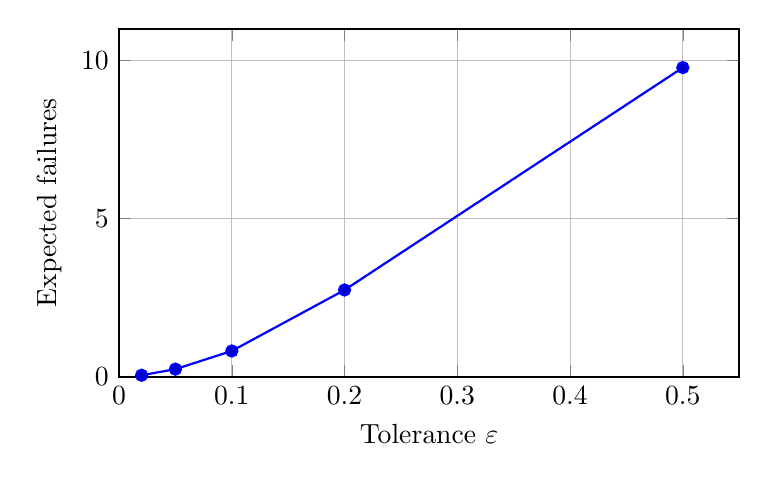
\begin{tikzpicture}
\begin{axis}[
  width=0.78\textwidth,
  height=6.0cm,
  xlabel={Tolerance \(\varepsilon\)},
  ylabel={Expected failures},
  xmin=0, xmax=0.55,
  ymin=0, ymax=11,
  grid=both,
  thick
]
\addplot coordinates {(0.02,0.046) (0.05,0.238) (0.10,0.813) (0.20,2.741) (0.50,9.773)};
\end{axis}
\end{tikzpicture}
\caption{Expected failures against the chance-constraint tolerance on the eight-book wear sweep. Loosening the veto lets the worn machines run and the failure count returns.}
\label{fig:eps}
\end{figure}

Tightening \(\varepsilon\) from \(0.50\) to \(0.02\) cuts expected failures from \(9.77\) to \(0.05\) and raises the maintenance count from \(7.0\) to \(15.0\). Makespan moves from \(1336\) minutes down to \(1145\), not up. Energy moves with it, from \(228.6\,\mathrm{kWh}\) down to \(182.0\,\mathrm{kWh}\). On this wear parameterisation, a sixteen-minute renewal is cheap relative to the repair delay and the slowed cycles it prevents, all the way to the tightest tolerance tested. The knob behaves as a knob. It does not, inside the tested interval, produce the rising makespan that a much longer maintenance, or a much healthier fleet, would produce. That qualification belongs in the result. The technology exposes \(\varepsilon\) so that a plant with different renewal costs can set it from its own curve rather than from this one.

\subsection{A static evolutionary reference}

On four nominal books the small NSGA-II, without maintenance, produced nondominated sets of size \(14\), \(16\), \(7\), and \(18\). The best makespan in those four sets was \(1002\), \(1274\), \(1081\), and \(1219\) minutes. The best tardiness was \(649\), \(131\), \(571\), and \(326\) minutes. The best energy was \(204\), \(263\), \(237\), and \(238\,\mathrm{kWh}\). These are four separate single-book searches. A point that holds the best makespan of a front is not the point that holds the best tardiness of that front.

The reference is useful as a ceiling check and as a warning against a sloppy comparison. On one book, a population that can see every order at time zero can reach a makespan near \(1000\) minutes without any maintenance, which is in the neighbourhood of the full system's twenty-book mean of \(1052\). The energy attached to the evolutionary fronts does not enter the neighbourhood of \(168\,\mathrm{kWh}\), and the search has no failure action to bring it there. Giving the evolutionary method the maintenance map and a long enough population would be a different experiment. It was not run. The online system does not need that population at dispatch time, which is the operational distinction drawn in Section~\ref{sec:tech1-review} and left intact by these four fronts.

\subsection{Where the gain comes from}

The four scenarios support a single decomposition.

The classical rules are not close to each other, and the estimation does not replace them with a vague ``heuristic baseline.'' Earliest due date is the tardiness rule. Shortest processing time is the energy rule among the four, because it happens to favour shorter occupations on lighter machines more often than earliest due date does. First-in-first-out is the rule that shows the cost of having no score at all. Apparent tardiness cost does not dominate earliest due date once health-scaled processing times and colour setups are in the cell.

The graph score without maintenance, RCH, is responsible for a first cut of roughly \(250\) to \(350\) minutes of makespan and roughly \(50\) to \(100\,\mathrm{kWh}\), depending on the scenario, together with a partial reduction in expected failures. It does this while remaining competitive with earliest due date on nominal tardiness and clearly better than earliest due date on rush and wear tardiness. That is the estimate of resource-coupled attention on this cell. The resource half of the name is the smaller half. The attention is mostly using health, energy, slack, and processing time. Contention features add a modest, correctly signed shift when lots are short.

The twin is responsible for the second cut: failures from about ten, or about thirty in the wear scenario, down to about one, and a further several hundred minutes of makespan. The mechanism matches Table~\ref{tab:worked} extended over the day. Maintenance is a local cost. Avoided repair delay and restored machine speed are a global saving. The no-status ablation shows that merely penalising health inside \(\psi\), without the authority to renew the machine, captures only the first cut.

Preference conditioning was not re-identified at the corners of the simplex, and a gate sweep at the balanced coefficients did not move energy and tardiness in clean opposite directions. The estimation does not claim a traced Pareto front from those gates. What it claims is a scalarised policy at a stated \(\omega\), plus a tolerance \(\varepsilon\) that does trace a front between failures and maintenance count. A plant that wants a different compromise between makespan and energy can re-run Algorithm~\ref{alg:cem} at a new \(\omega\). The identification is short on this cell. Pretending that the present gates already provide that compromise would not match the runs.

\subsection{Spreads, and which gaps survive them}

Means without spreads invite a false ranking. Table~\ref{tab:nominal-std} gives the twenty-book standard deviations for the nominal scenario. The same qualitative pattern holds in the other three scenarios: makespan and energy under the full system are tighter as well as smaller, and tardiness is wide for everyone.

\begin{table}[ht]
\centering
\caption{Standard deviations on the twenty nominal books. Compare with the means in Table~\ref{tab:nominal}.}
\label{tab:nominal-std}
\small
\begin{tabular}{lrrrr}
\toprule
Method & Makespan & Tardiness & Energy & Failures \\
\midrule
FIFO & 165.5 & 703.0 & 35.0 & 3.29 \\
SPT & 229.6 & 571.9 & 40.8 & 3.81 \\
EDD & 175.2 & 355.5 & 39.7 & 3.48 \\
ATC & 188.2 & 410.7 & 37.6 & 3.29 \\
RCH & 146.3 & 250.5 & 28.6 & 2.25 \\
RCH-SSDT & 83.4 & 204.5 & 19.4 & 0.15 \\
No resource & 106.8 & 139.2 & 21.1 & 0.15 \\
No status & 179.2 & 282.8 & 24.3 & 2.00 \\
\bottomrule
\end{tabular}
\end{table}

A gap survives the spread when it is large next to both standard deviations, not when a \(t\)-test has been performed. No paired test is reported, and one should not be invented from the two margins. The comparisons that survive on that rough standard are these.

Makespan of RCH-SSDT against any classical rule, in every scenario. The nominal gap is about \(470\) minutes against a classical spread of \(150\) to \(230\) and a full-system spread of \(83\). The wear gap is about \(900\) minutes. The rush gap is about \(700\) minutes.

Energy of RCH-SSDT against any classical rule, in every scenario. The nominal gap against the best classical energy, shortest processing time, is about \(100\,\mathrm{kWh}\), against spreads of \(41\) and \(19\).

Expected failures of RCH-SSDT against every method that is not allowed to maintain. The nominal drop is from the teens to \(0.91\), with a full-system spread of \(0.15\). This is the cleanest column in the thesis.

Imbalance of RCH and of RCH-SSDT against the classical rules. The nominal drop is from about \(370\) to \(222\) or \(260\), and the full-system spread is \(27\) minutes of standard deviation. The load weight \(5.660\) in Equation~\eqref{eq:wstar} is the coefficient that produces this column.

RCH without maintenance against first-in-first-out on makespan and energy. The makespan gap of \(286\) minutes is larger than either spread, though less dramatic than the gap that appears once maintenance is allowed.

The comparisons that do not survive are equally part of the estimate. Nominal tardiness of RCH-SSDT against earliest due date is \(165\) against \(212\), with spreads \(205\) and \(356\). The point estimate favours the full system. A single unlucky book can reverse it. Nominal on-time rate, \(0.90\) against \(0.89\), is a tie. The resource ablation against the full system on the nominal book is a tie, and on the shortage book it is a shift of about \(36\) minutes of makespan against spreads near \(90\). Calling that shift a proved saving would over-read twenty books. Calling it noise would ignore that the sign is the same under rush and under shortage and is absent under wear, which is the pattern a real but small token effect would leave.

The full system is also more repeatable. Its makespan spread is about half the classical spread. Part of that tightness is mechanical: preventive maintenance removes the long random-looking repair delays that inflate some books and not others, even though those delays are expectations rather than draws. A method that sometimes accepts eight expected failures and sometimes accepts twenty-five will have a wide makespan. A method that holds the expected count near one will not. Repeatability is a target the problem statement did not list, and the tables give it anyway.

\subsection{What the weights say about the tables}

Equation~\eqref{eq:wstar} and Table~\ref{tab:weights} were identified before any estimation book was generated. They predict the tables more specifically than the architecture diagram does.

The largest weight is load deviation. Every scenario shows a lower imbalance for RCH than for the classical rules, and the full system lowers it further because renewed machines can take work that a worn machine would otherwise hoard and then lose to a repair. The second-largest relevant weights, skill gap and failure probability, are why a machine-only reading of the graph is the wrong reading. Skill never enters the classical rules except as a longer processing time after a weak pairing has already been chosen. Failure never enters them at all.

The smallest weight is colour contention. The shortage scenario was built to make that weight visible, and the visibility is modest. This is consistent rather than contradictory. A weight of \(0.133\) cannot move a day by the same amount as a weight of \(5.660\) or as a sixteen-minute renewal that deletes a forty-eight-minute expected repair. Die contention, at \(0.917\), is large enough to matter when both cutters want a die, and the nominal cell has two dies for two cutters, so the feature is often slack. A cell with one die would be a different estimate.

Setup weight \(1.029\) shows up as fewer colour changes: \(57.8\) under first-in-first-out and \(57.6\) under earliest due date, against \(43.2\) under the full system on the nominal book. Earliest due date groups nothing by colour. The score does, unless a due date or a health veto says otherwise. The reduction is about fifteen setups, each eleven minutes, which is \(165\) minutes of setup time returned to the day. That is a real slice of the makespan gap and it is not the whole gap. The rest is routing toward healthier, less loaded machines, and, for the full system, the repair time that is no longer charged.

\subsection{What a factory would instrument first}

The estimate implies an order of instrumentation, and the order is not the order in which the technologies were named.

The first instrument is a health indicator on the automatic cutter, the embroidery head, and the more worn lockstitch, mapped onto the unit interval that Equation~\eqref{eq:ptime} expects. Those three machines dominate power or dominate the route. A health number that cannot veto a cycle is a dashboard. The veto is Algorithm~\ref{alg:ssdt}, and it needs a maintenance action the operator is allowed to start without a separate work order. Sixteen minutes is the action this cell used. A plant whose knife change takes forty minutes should rerun the tolerance sweep before copying \(\varepsilon = 0.10\).

The second instrument is the operator skill table and a live free-time for each person. The skill weight is large, and the mask is what keeps Sew-3 off the bartack. A scheduler that knows machines and not people will reproduce the hidden wait described in Section~\ref{sec:rch}.

The third instrument is the die pool and the thread lots. They are cheap to count and they are already in the graph. On a one-day book of this size they are not where the hours are. They become first-priority only if a colour is routinely single-sourced and the due dates on that colour are the ones the planner is missing. The shortage table is the test: if a factory's own version of that table shows a large gap between the full score and the no-resource score, the lots are the constraint. If the gap looks like the thirty-minute shift reported here, the lots are not the constraint.

The network of Equations~\eqref{eq:gat-full} and \eqref{eq:gat-update} is not on this list. Nothing in the twenty-book cell is large enough to need a multi-layer embedding. The list is health with authority to maintain, then people, then tokens, and a deeper network only when the identification of twenty coefficients stops being enough. That is a smaller system than a generic Industry~4.0 diagram, and it is the system the numbers support.

\subsection{A note on the clock}

All times in the tables are minutes from the release of the first order. A nominal makespan of \(1052\) minutes is about \(17.5\) hours, longer than a single staffed shift. The cell as parameterised is a congested day-and-evening load: one embroidery head, one hardware bench, and a worn fast cutter. The absolute clock is a property of those capacities and of the batch sizes, not a claim that a school-bag plant cannot finish sixteen orders in a shift. A plant with two embroidery heads would show a shorter clock and, if the cutter were healthy, a smaller maintenance effect. The ratios are what the estimate is for. The full system is about thirty percent shorter than first-in-first-out on the nominal book (\(1521\) to \(1052\)) and about forty-five percent shorter on the wear book (\(2098\) to \(1122\)). Those ratios are the quantities a different capacity would be expected to preserve in direction, not in minutes.

Energy should be read the same way. One hundred and sixty-eight kilowatt-hours for the nominal full system is the cutter, the embroidery head, and the sewing machines over that long clock, including setups and the few maintenances. It is not a utility bill for a named factory. It is the integral of the nameplate powers in Table~\ref{tab:machines} under the wear surcharge. Moving work off Cutter-A is the main reason the integral falls. A plant whose automatic cutter is efficient when worn would see a smaller energy gap and would still see the failure gap, because the hazard does not depend on the nameplate.

\subsection{The four questions, answered in one table}

Section~\ref{sec:problem-set} asked four questions. Table~\ref{tab:summary} answers them as ratios, so the four scenarios can sit on one page. The ratio is the full system divided by the named baseline. A ratio below one is an improvement.

\begin{table}[ht]
\centering
\caption{RCH-SSDT divided by a baseline, four scenarios. Makespan and failures are against first-in-first-out. Energy is against shortest processing time, the best classical energy. Tardiness is against earliest due date, the best classical due-date rule. Ratios use the means of Tables~\ref{tab:nominal}--\ref{tab:shortage}.}
\label{tab:summary}
\small
\begin{tabular}{lrrrr}
\toprule
Scenario & Makespan / FIFO & Tardiness / EDD & Energy / SPT & Failures / FIFO \\
\midrule
Nominal & 0.69 & 0.78 & 0.62 & 0.05 \\
Rush & 0.63 & 0.27 & 0.60 & 0.03 \\
Wear & 0.53 & 0.16 & 0.50 & 0.02 \\
Shortage & 0.71 & 0.65 & 0.63 & 0.05 \\
\bottomrule
\end{tabular}
\end{table}

The first question was whether the coupled system could cut makespan, energy, and failures without giving the due-date rule a large tardiness advantage. On the nominal book the makespan ratio is \(0.69\), the energy ratio is \(0.62\), and the failure ratio is \(0.05\). The tardiness ratio against earliest due date is \(0.78\) as a ratio of means, and Section~\ref{sec:estimate} has already said that this particular ratio sits inside a wide spread. The system does not buy its energy by missing the promises the due-date rule was keeping. It also does not earn a precise claim to have beaten that rule on tardiness.

The second question was whether the same system holds under stress. The wear row is the strongest answer: makespan ratio \(0.53\), tardiness ratio \(0.16\), energy ratio \(0.50\), failure ratio \(0.02\). The rush row is the next strongest, especially on tardiness, where earliest due date sees the new orders and still finishes them late because the machines it prefers are the ones accumulating repair delay. The shortage row looks like the nominal row. Tight thread lots change the feasible set. They do not change the ranking of the technologies.

The third question was which technology produces which gain. The ratios in Table~\ref{tab:summary} are the coupled system. The ablations, which do not fit in the ratio table, split it. Removing maintenance returns failures from about one to about ten on the nominal book and to about thirty on the wear book, and it gives back a few hundred minutes of makespan. Removing resource features does not. The first technology, as identified, is a load-aware, skill-aware, health-aware score. The second technology is the action that renews health. Both are required for the failure column. Only the first is required for a large part of the imbalance column.

The fourth question was whether \(\varepsilon\) is a real knob. Table~\ref{tab:eps} is the answer, and it is monotone in the direction the chance constraint predicts: a tighter tolerance, more maintenances, fewer expected failures, and, on this wear parameterisation, a shorter rather than a longer day. A plant with a slower tool change would be expected to find a bottom in that curve. This plant, inside the tested range, did not.

A fifth question was left soft on purpose. Tardiness ratios in the nominal and shortage rows should be read as ``no damage to the due-date rule, inside a large book-to-book spread.'' Tardiness ratios in the rush and wear rows are large enough to survive that spread. The soft question is therefore not one answer. It depends on whether the day is being lost to wear and rush, or only to ordinary congestion.

\subsection{Limits of the estimate}

The cell is a simulator with a known wear recursion. A physical embroidery head has a health indicator that must be built from thread-break counts, temperature, and current, with the measurement path reviewed by Lei and co-authors \cite{lei2018}, and it has a Kalman residual that this estimate sets to zero. If that residual is large, the veto will chatter, and the sixteen-minute maintenance will be applied to noise. The formula for dealing with the residual is Equation~\eqref{eq:kalman-upd}. It was not exercised.

The order books contain sixteen or twenty orders and nine machines. Graph policies are attractive in the literature because they transfer to larger books \cite{zhang2020,song2023}. This estimate does not test that transfer. A coefficient vector identified on sixteen-order books is not, on the evidence here, a policy for a plant with two hundred machines. The multi-layer model of Equations~\eqref{eq:gat-full} and \eqref{eq:gat-update} is the form proposed for that plant, and it is untested in these tables.

Expected failures are not random failures. Inserting the mean repair delay makes methods comparable and removes the variance of a single Bernoulli draw. It also makes the timeline optimistic about clustering. Two failures that the expectation treats as independent half-repairs can, in a real morning, land on the same operator and block the bartack for a full repair plus the queue behind it. A stochastic replication would widen the spreads. It would not, unless the intensity model is badly wrong, reverse a gap between one expected failure and thirty.

Tardiness is a noisy sum. The nominal comparison with earliest due date should be read as ``no harm, within a large spread,'' not as a precise percentage. The wear and rush comparisons are the ones in which tardiness actually moves.

Resource coupling is real in the model and small in the estimate. That is the right outcome to publish. Inflating it to match the size of the maintenance effect would mislead a factory into instrumenting thread lots before instrumenting cutter wear. The instrumentation order implied by these tables is the other way around: health and the authority to act on health first, token contention second, and a deeper network only when the cell is larger than the one these coefficients were fit to.

The evolutionary reference is too small to be a competitor. It is a sanity check. A serious NSGA-III run of the kind Gong and co-authors used for five objectives \cite{gong2019}, with maintenance included in the chromosome, remains an open comparison and would be the right offline partner for the online policy.

The questions in Section~\ref{sec:problem-set} can be answered in one further sentence each, now that the ratios and the spreads are both on the page. The coupled system does cut makespan, energy, imbalance, and expected failures relative to the four rules, and on a nominal book it does not hand those rules a tardiness advantage that survives the spread. Under rush and under accelerated wear the same system holds, and tardiness moves with the makespan because the lateness was being produced by repair delay. The ablation that removes maintenance gives back the failure column and a large part of the makespan; the ablation that removes resource features does not. The tolerance \(\varepsilon\) trades maintenances against expected failures in the predicted direction. Those four sentences are the estimate. Everything else in the section is the condition under which they were measured.

Table~\ref{tab:seeds} fixes the seeds so that a rerun is a comparison and not a new experiment. Changing a seed changes the order book. Changing a parameter changes the cell. Either change is allowed, and neither is what the tables already report.

\begin{table}[ht]
\centering
\caption{Seeds used by the driver. Estimation seeds are paired across every method.}
\label{tab:seeds}
\small
\begin{tabular}{ll}
\toprule
Role & Seeds \\
\midrule
Identification books & 11, 23, 37, 41 \\
Nominal, rush, wear, shortage & 1000 to 1019 \\
Tolerance sweep, wear only & 4000 to 4007 \\
Evolutionary reference & 5000 to 5003 \\
\bottomrule
\end{tabular}
\end{table}

The runs are reproducible from the thesis directory. The cell, the score, the identification, and the comparison driver are the program \texttt{simulation/shop\_sim.py}. Training books are seeds \(11\), \(23\), \(37\), and \(41\). Estimation books are seeds \(1000\) through \(1019\). The tolerance sweep uses seeds \(4000\) through \(4007\) on the wear scenario. The evolutionary reference uses seeds \(5000\) through \(5003\). The coefficient vector is written beside the tables in \texttt{data/results.json}. A reader who changes \(\varepsilon\), a wear coefficient, or a token capacity and reruns the driver will get a different table, and that is the intended use of the program. The numbers in this chapter are the numbers that driver produced for the parameterisation written down in Section~\ref{sec:build}.

Nothing in the tables comes from a school that can be visited. The routes, the powers, and the wear rates are a constructed cell, documented so that the runs can be repeated. The technologies are estimated on that cell. The estimate supports the design: a masked resource-bundle score shortens and cools the day, and a chance-constrained renewal of machine health is what keeps the day from being spent inside expected repairs. It does not support a claim about a particular factory's next quarter.

What the cell does support is a decision about where to spend the next engineering month. Put a health indicator and a sixteen-minute maintenance authority on the worn, high-power machines before building a deeper network and before instrumenting every thread lot. Keep the operator skill table in the mask, because an infeasible bartack assignment is a hidden wait. Treat colour contention as a feature that is present and, on this book, nearly inactive, and re-identify if a future book shows the shortage gap growing past the spreads in Table~\ref{tab:nominal-std}. Leave \(\varepsilon\) visible. The wear sweep is the evidence that the number matters, and it is also the evidence that the right number depends on how long a renewal takes. A scheduler that hides the tolerance inside a trained weight cannot be retuned when the knife-change time changes. The system in this thesis can.
